\documentclass[xetex,mathserif,serif,aspectratio=169]{beamer}

\usepackage{xltxtra}
\usepackage{color}
\usepackage{url}
\usepackage{listings}
\usepackage{fontspec}
\usepackage{geometry}
\usepackage{lastpage}
\usepackage{fancyhdr}
\usepackage{amsmath}
\usepackage{amsthm}
\usepackage{amssymb}
\usepackage{blkarray}
\usepackage{multicol}
\usepackage{relsize}
\usepackage{listings}
\usepackage{xunicode}
\usepackage{xltxtra}
\usepackage{color}
\usepackage{url}
\usepackage{courier}

\usefonttheme[onlymath]{serif}

\definecolor{solarized@base03}{HTML}{002B36}
\definecolor{solarized@base02}{HTML}{073642}
\definecolor{solarized@base01}{HTML}{586e75}
\definecolor{solarized@base00}{HTML}{657b83}
\definecolor{solarized@base0}{HTML}{839496}
\definecolor{solarized@base1}{HTML}{93a1a1}
\definecolor{solarized@base2}{HTML}{EEE8D5}
\definecolor{solarized@base3}{HTML}{FDF6E3}
\definecolor{solarized@yellow}{HTML}{B58900}
\definecolor{solarized@orange}{HTML}{CB4B16}
\definecolor{solarized@red}{HTML}{DC322F}
\definecolor{solarized@magenta}{HTML}{D33682}
\definecolor{solarized@violet}{HTML}{6C71C4}
\definecolor{solarized@blue}{HTML}{268BD2}
\definecolor{solarized@cyan}{HTML}{2AA198}
\definecolor{solarized@green}{HTML}{859900}
\definecolor{yaleblue}{HTML}{0E4C92}

\newcommand{\yellow}[1]{\textcolor{solarized@yellow}{#1}}
\newcommand{\orange}[1]{\textcolor{solarized@orange}{#1}}
\newcommand{\red}[1]{\textcolor{solarized@red}{#1}}
\newcommand{\magenta}[1]{\textcolor{solarized@magenta}{#1}}
\newcommand{\violet}[1]{\textcolor{solarized@violet}{#1}}
\newcommand{\blue}[1]{\textcolor{solarized@blue}{#1}}
\newcommand{\cyan}[1]{\textcolor{solarized@cyan}{#1}}
\newcommand{\green}[1]{\textcolor{solarized@green}{#1}}
\newcommand{\yblue}[1]{\textcolor{yaleblue}{#1}}
\newcommand{\base}[1]{\textcolor{solarized@base01}{#1}}

\newcommand{\dfont}[1]{\fontspec[Ligatures={Common}]{Didot}\fontsize{12pt}{15pt}\color{solarized@base02}\selectfont #1}%

\newcommand{\stitle}[1]{\textbf{\textcolor{solarized@blue}{#1}}}

\lstset{basicstyle=\footnotesize\ttfamily,breaklines=true}

\defaultfontfeatures{Mapping=tex-text}
\hypersetup{pdfstartview={FitH}}


\fontspec[Ligatures={Common}]{Didot}\fontsize{12pt}{15pt}\color{solarized@base02}\selectfont

\setbeamertemplate{navigation symbols}{}
\setbeamertemplate{footline}[text line]{%
  \parbox{0.99\linewidth}{
    \normalsize\vspace*{-24pt}\hfill{\color{solarized@base00}\insertframenumber/\inserttotalframenumber}
  }
}

\setlength{\parindent}{0pt}
\setlength{\parskip}{12pt}

\setbeamercolor{structure}{bg=solarized@base3, fg=solarized@base02}
\setbeamercolor{titlelike}{fg=solarized@cyan}
\setbeamercolor{title}{fg=solarized@blue}
\setbeamercolor{subtitle}{fg=solarized@magenta}
\setbeamercolor{alerted text}{fg=orange}
\setbeamercolor{itemize}{fg=solarized@base02}
\setbeamercolor{background canvas}{bg=solarized@base3}
\setbeamercolor{enumerate subitem}{fg=solarized@base02}

\newcommand{\minimize}{\mathop{\mathrm{minimize}}}
\newcommand{\argmin}{\mathop{\mathrm{arg\,min}}}
\newcommand{\argmax}{\mathop{\mathrm{arg\,max}}}
\newcommand{\st}{\mathop{\mathrm{subject\,\,to}}}

\lstset{ %
  language=R,                     % the language of the code
  basicstyle=\footnotesize,       % the size of the fonts that are used for the code
  numbers=left,                   % where to put the line-numbers
  numberstyle=\tiny\color{gray},  % the style that is used for the line-numbers
  stepnumber=1,                   % the step between two line-numbers. If it's 1, each line
                                  % will be numbered
  numbersep=5pt,                  % how far the line-numbers are from the code
  backgroundcolor=\color{white},  % choose the background color. You must add \usepackage{color}
  showspaces=false,               % show spaces adding particular underscores
  showstringspaces=false,         % underline spaces within strings
  showtabs=false,                 % show tabs within strings adding particular underscores
  frame=single,                   % adds a frame around the code
  rulecolor=\color{black},        % if not set, the frame-color may be changed on line-breaks within not-black text (e.g. commens (green here))
  tabsize=2,                      % sets default tabsize to 2 spaces
  captionpos=b,                   % sets the caption-position to bottom
  breaklines=true,                % sets automatic line breaking
  breakatwhitespace=false,        % sets if automatic breaks should only happen at whitespace
  title=\lstname,                 % show the filename of files included with \lstinputlisting;
                                  % also try caption instead of title
  keywordstyle=\color{solarized@blue},      % keyword style
  commentstyle=\color{solarized@green},   % comment style
  stringstyle=\color{solarized@magenta},      % string literal style
  escapeinside={\%*}{*)},         % if you want to add a comment within your code
  morekeywords={*,...}            % if you want to add more keywords to the set
}

\title{MATH 209: Course Introduction}
\author{Taylor B. Arnold}

\begin{document}

\dfont

%%%%%%%%%%%%%%%%%%%%%%%%%%%%%%%%%%%%%%%%%%%%%%%%%%%
\begin{frame}[fragile]

\vfill

{\fontsize{0.7cm}{0cm}\selectfont \blue{Math 209\\ \vspace{14pt} \hspace{1cm}
Introduction to Statistical Modeling} }\\\vspace{0.5cm}

\vspace{2cm}

Taylor Arnold \\
e-mail: tarnold2@richmond.edu
\end{frame}

% %%%%%%%%%%%%%%%%%%%%%%%%%%%%%%%%%%%%%%%%%%%%%%%%%%%
% \begin{frame}[fragile]

% \stitle{MATH 209 Introduction to Statistical Modeling} \vspace{12pt}

% From the catalog:

% \begin{quote}
% Topics will include exploratory data analysis, correlation, linear
% and multiple regression, design of experiments, basic probability,
% the normal distribution, sampling distributions, estimation,
% hypothesis testing and randomization approach to inference.
% Exploratory graphical methods, model building and model checking
% techniques will be emphasized with extensive use of statistical
% software for data analysis.
% \end{quote}

% \end{frame}

% % %%%%%%%%%%%%%%%%%%%%%%%%%%%%%%%%%%%%%%%%%%%%%%%%%%%
% % \begin{frame}[fragile]

% % In 2009, Val Varian, Google’s Chief Economist, said:

% % \begin{quote}
% % I keep saying the sexy job in the next ten years will be
% % statisticians\ldots and I’m not kidding!
% % \end{quote}

% % \end{frame}

% % %%%%%%%%%%%%%%%%%%%%%%%%%%%%%%%%%%%%%%%%%%%%%%%%%%%
% % \begin{frame}[fragile]

% % \begin{center}
% % 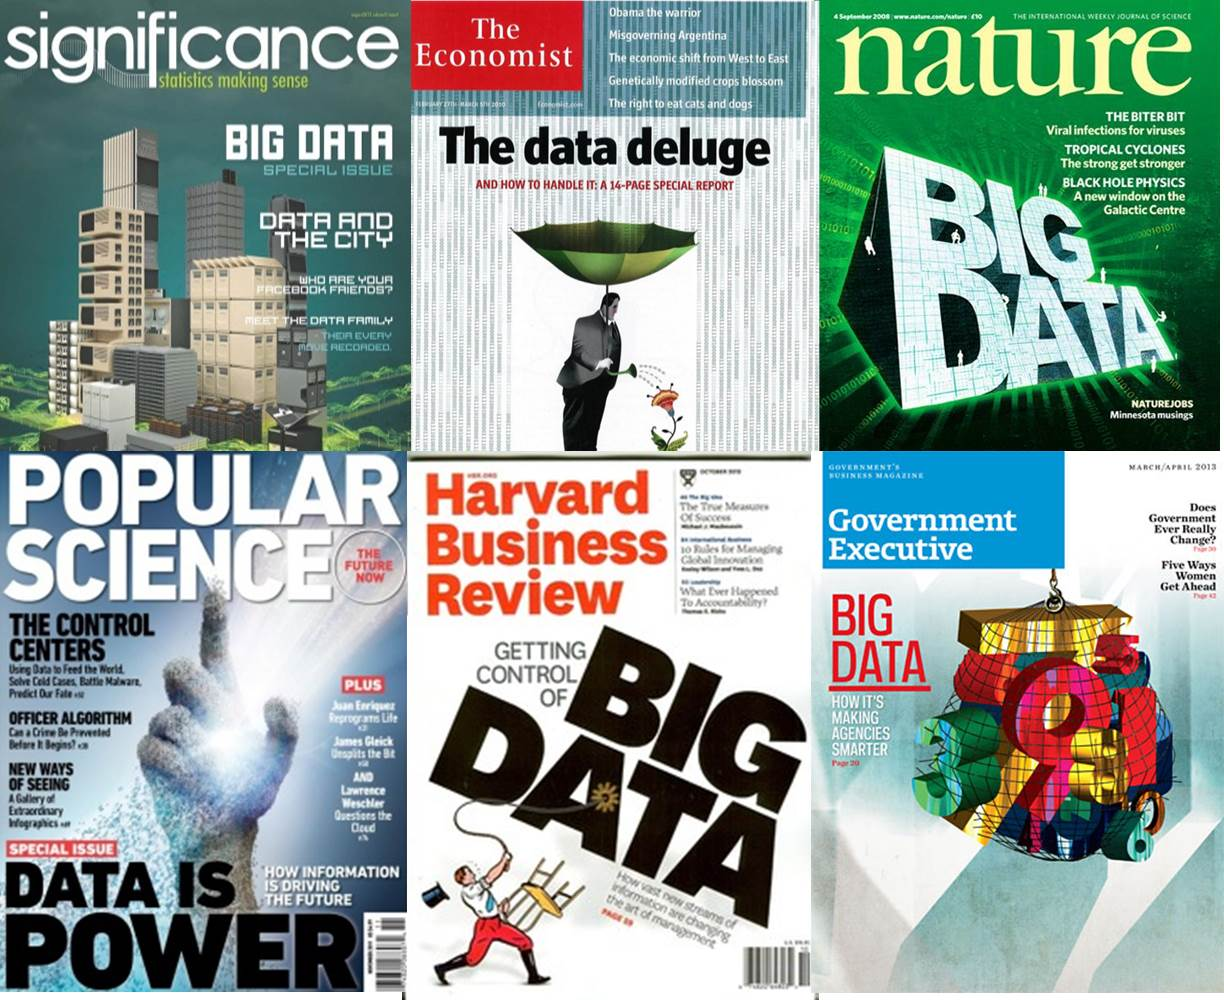
\includegraphics[height=0.85\textheight]{img/Big-Data-Magazine-covers.jpg}
% % \end{center}

% % \end{frame}

% % %%%%%%%%%%%%%%%%%%%%%%%%%%%%%%%%%%%%%%%%%%%%%%%%%%%
% % \begin{frame}[fragile]

% % If you are here because you have been dying to hear about
% % the randomization approach to inference \magenta{that's great}!

% % \pause But, let's be honest, I assume many of you are taking
% % an introductory statistics course because its a prerequisite
% % for your major, required for graduate school, or strongly
% % recommended for continued study in some area of interest to
% % you. \pause \magenta{That's great too!}

% % \end{frame}

%%%%%%%%%%%%%%%%%%%%%%%%%%%%%%%%%%%%%%%%%%%%%%%%%%%
\begin{frame}[fragile] \frametitle{}

\noindent
\begin{minipage}{0.5\textwidth}
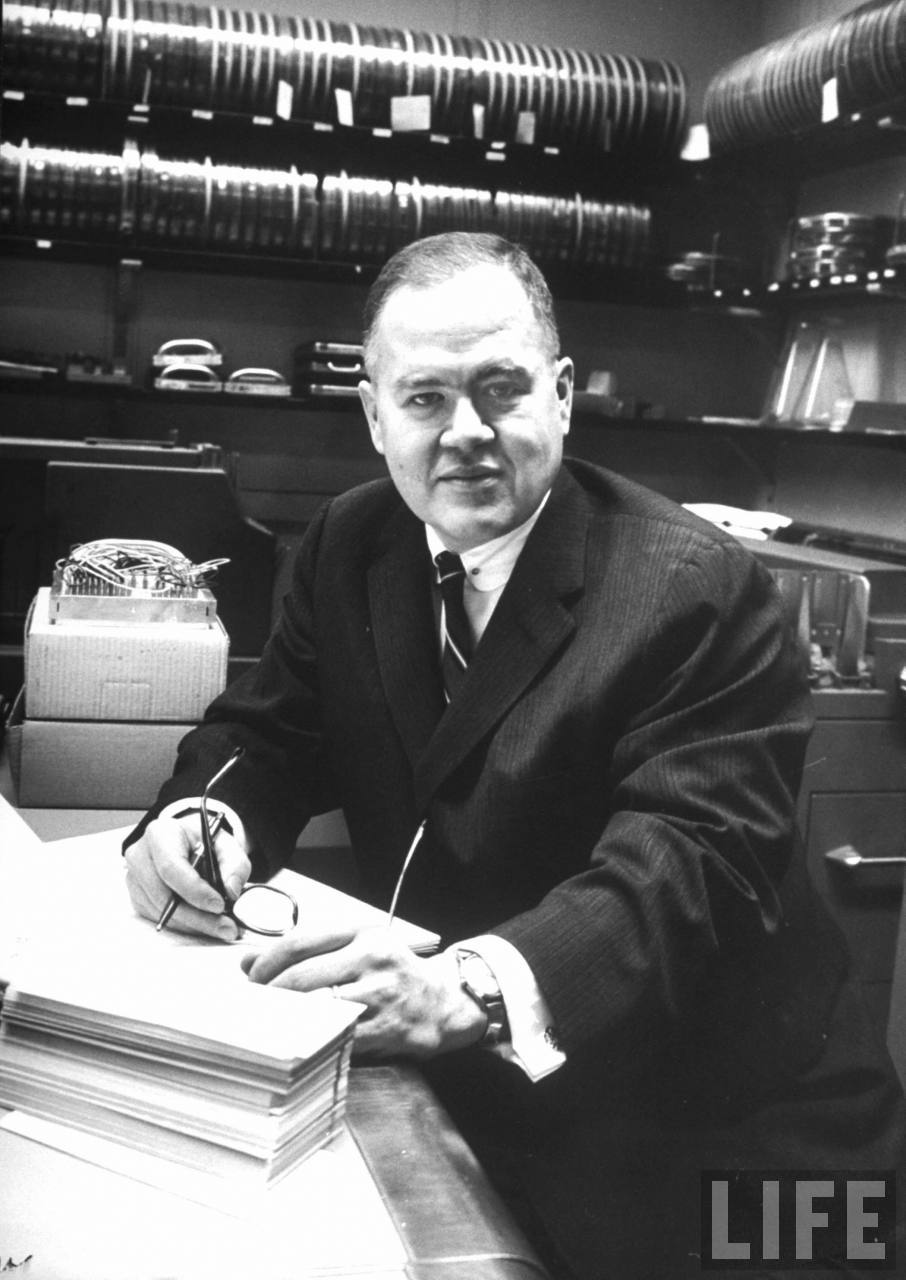
\includegraphics[width=0.9\linewidth]{img/tukey.jpg}
\end{minipage}%%% to prevent a space
\begin{minipage}{0.5\textwidth}
``The best thing about being a statistician is that
you get to play in everyone's backyard.'' \\

\hfill - John Tukey
\end{minipage}

\end{frame}

%%%%%%%%%%%%%%%%%%%%%%%%%%%%%%%%%%%%%%%%%%%%%%%%%%%
\begin{frame}[fragile]

I am an \magenta{applied statistician}. A sampling of projects and datasets
I have worked on include:
\begin{itemize}
\item cell phone telemetry
\item emergency room patient flow
\item finding holes in specialized medical coverage in rural US
\item Canadian court case citations
\item Olympic figure skating scoring
\item auto insurance risk factors
\item 170k documentary photographs from the 1930's
\item treatment outcomes for open-angle glaucoma
\item detecting radicalization from social media data
\item financial warfare
\end{itemize}

\end{frame}

%%%%%%%%%%%%%%%%%%%%%%%%%%%%%%%%%%%%%%%%%%%%%%%%%%%
\begin{frame}[fragile] \frametitle{}

\begin{flushright}
{\sc\fontsize{1cm}{0cm}\selectfont \textcolor{solarized@blue}{Statistics?}}
\end{flushright}

\end{frame}

%%%%%%%%%%%%%%%%%%%%%%%%%%%%%%%%%%%%%%%%%%%%%%%%%%%
\begin{frame}[fragile] \frametitle{}

Hans Rosling's 200 Countries, 200 Years, 4 Minutes - The Joy of Stats:
\begin{center}
\url{https://www.youtube.com/watch?v=jbkSRLYSojo}
\end{center}

\end{frame}

%%%%%%%%%%%%%%%%%%%%%%%%%%%%%%%%%%%%%%%%%%%%%%%%%%%
\begin{frame}[fragile]

New York Times: Gun homicides in New Zealand are about as common as deaths from
falling from a ladder in the United States.

\begin{center}
\url{http://nyti.ms/28yRifm}
\end{center}

\end{frame}

% %%%%%%%%%%%%%%%%%%%%%%%%%%%%%%%%%%%%%%%%%%%%%%%%%%%
% \begin{frame}[fragile]

% The Economist: The final bill, The legal storm surrounding banks is largely over

% \begin{center}
% \url{http://econ.st/2aWJFvH}
% \end{center}

% \end{frame}

%%%%%%%%%%%%%%%%%%%%%%%%%%%%%%%%%%%%%%%%%%%%%%%%%%%
\begin{frame}[fragile]

FiveThirtyEight: Steroids Probably Aren't Causing Baseball's Power Surge

\begin{center}
\url{http://53eig.ht/2aKodni}
\end{center}

\end{frame}

% %%%%%%%%%%%%%%%%%%%%%%%%%%%%%%%%%%%%%%%%%%%%%%%%%%%
% \begin{frame}[fragile] \frametitle{}

% \begin{flushright}
% {\sc\fontsize{1cm}{0cm}\selectfont \textcolor{solarized@blue}{Course Outline}}
% \end{flushright}

% \end{frame}

%%%%%%%%%%%%%%%%%%%%%%%%%%%%%%%%%%%%%%%%%%%%%%%%%%%
\begin{frame}[fragile]

\begin{center}
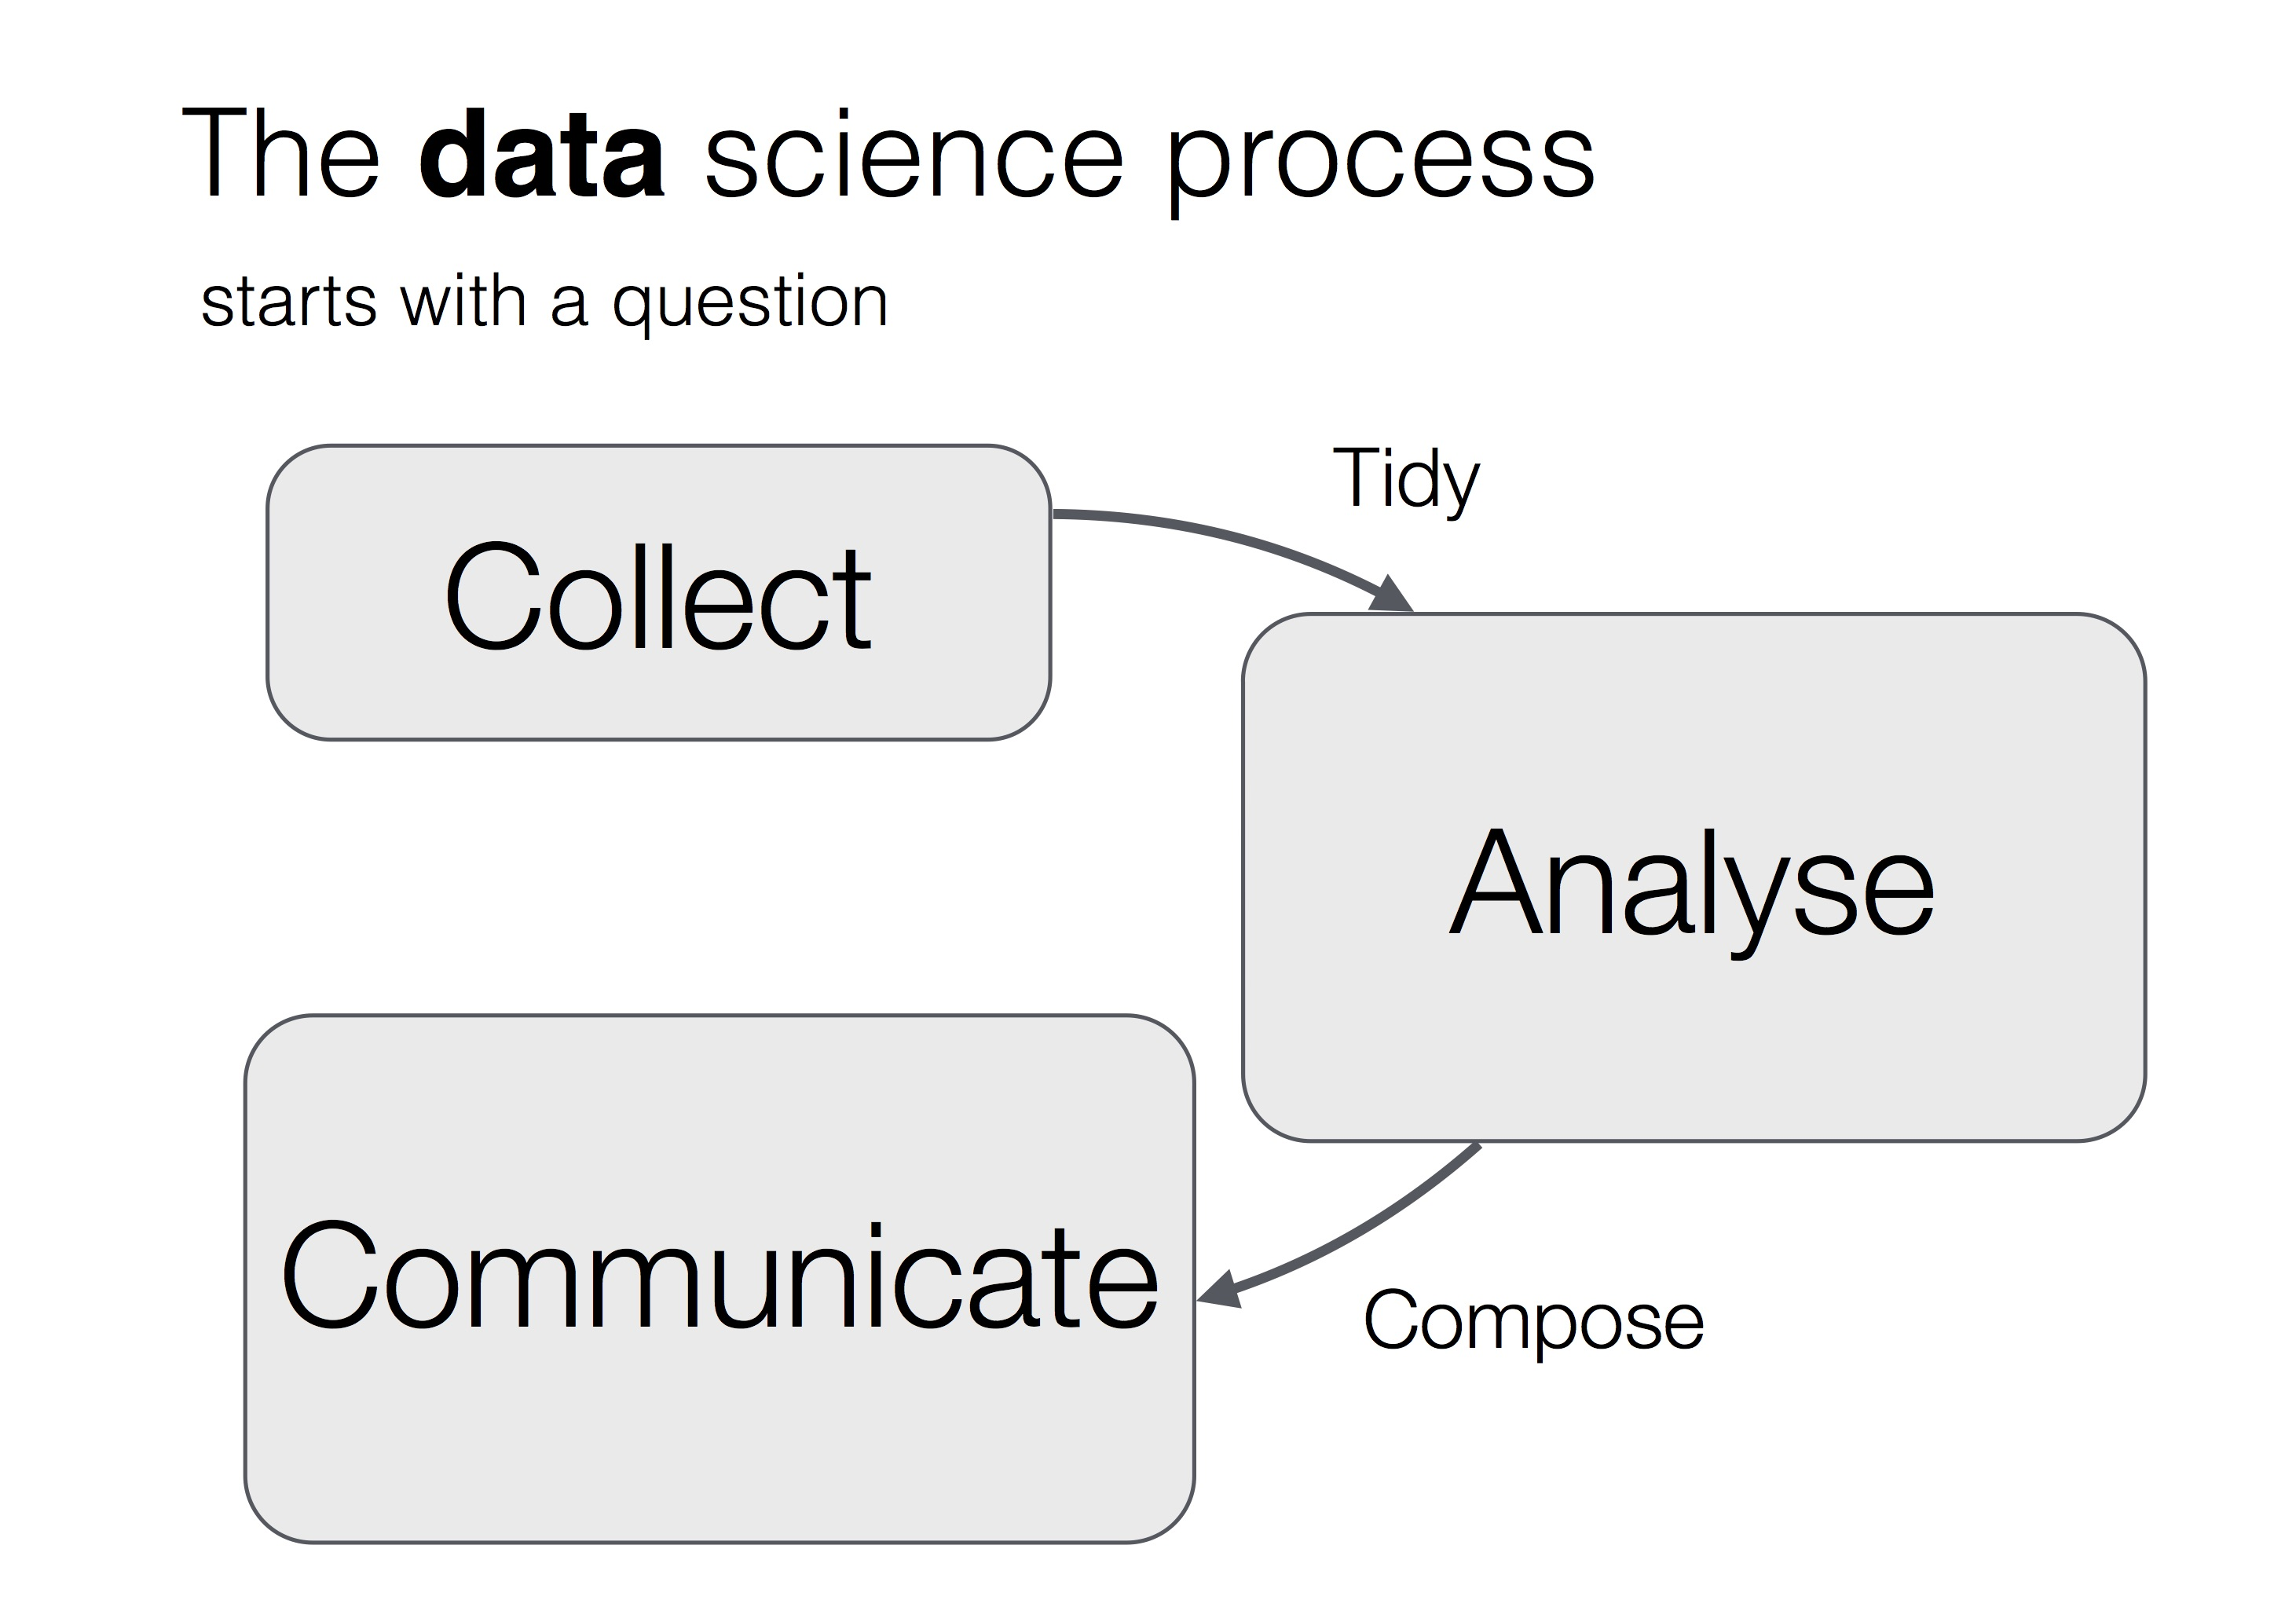
\includegraphics[height=0.8\textheight]{img/diagram01.jpg}
\end{center}

{\footnotesize diagram from Charlotte Wickham \url{http://stat511.cwick.co.nz/}}

\end{frame}

%%%%%%%%%%%%%%%%%%%%%%%%%%%%%%%%%%%%%%%%%%%%%%%%%%%
\begin{frame}[fragile]

\begin{center}
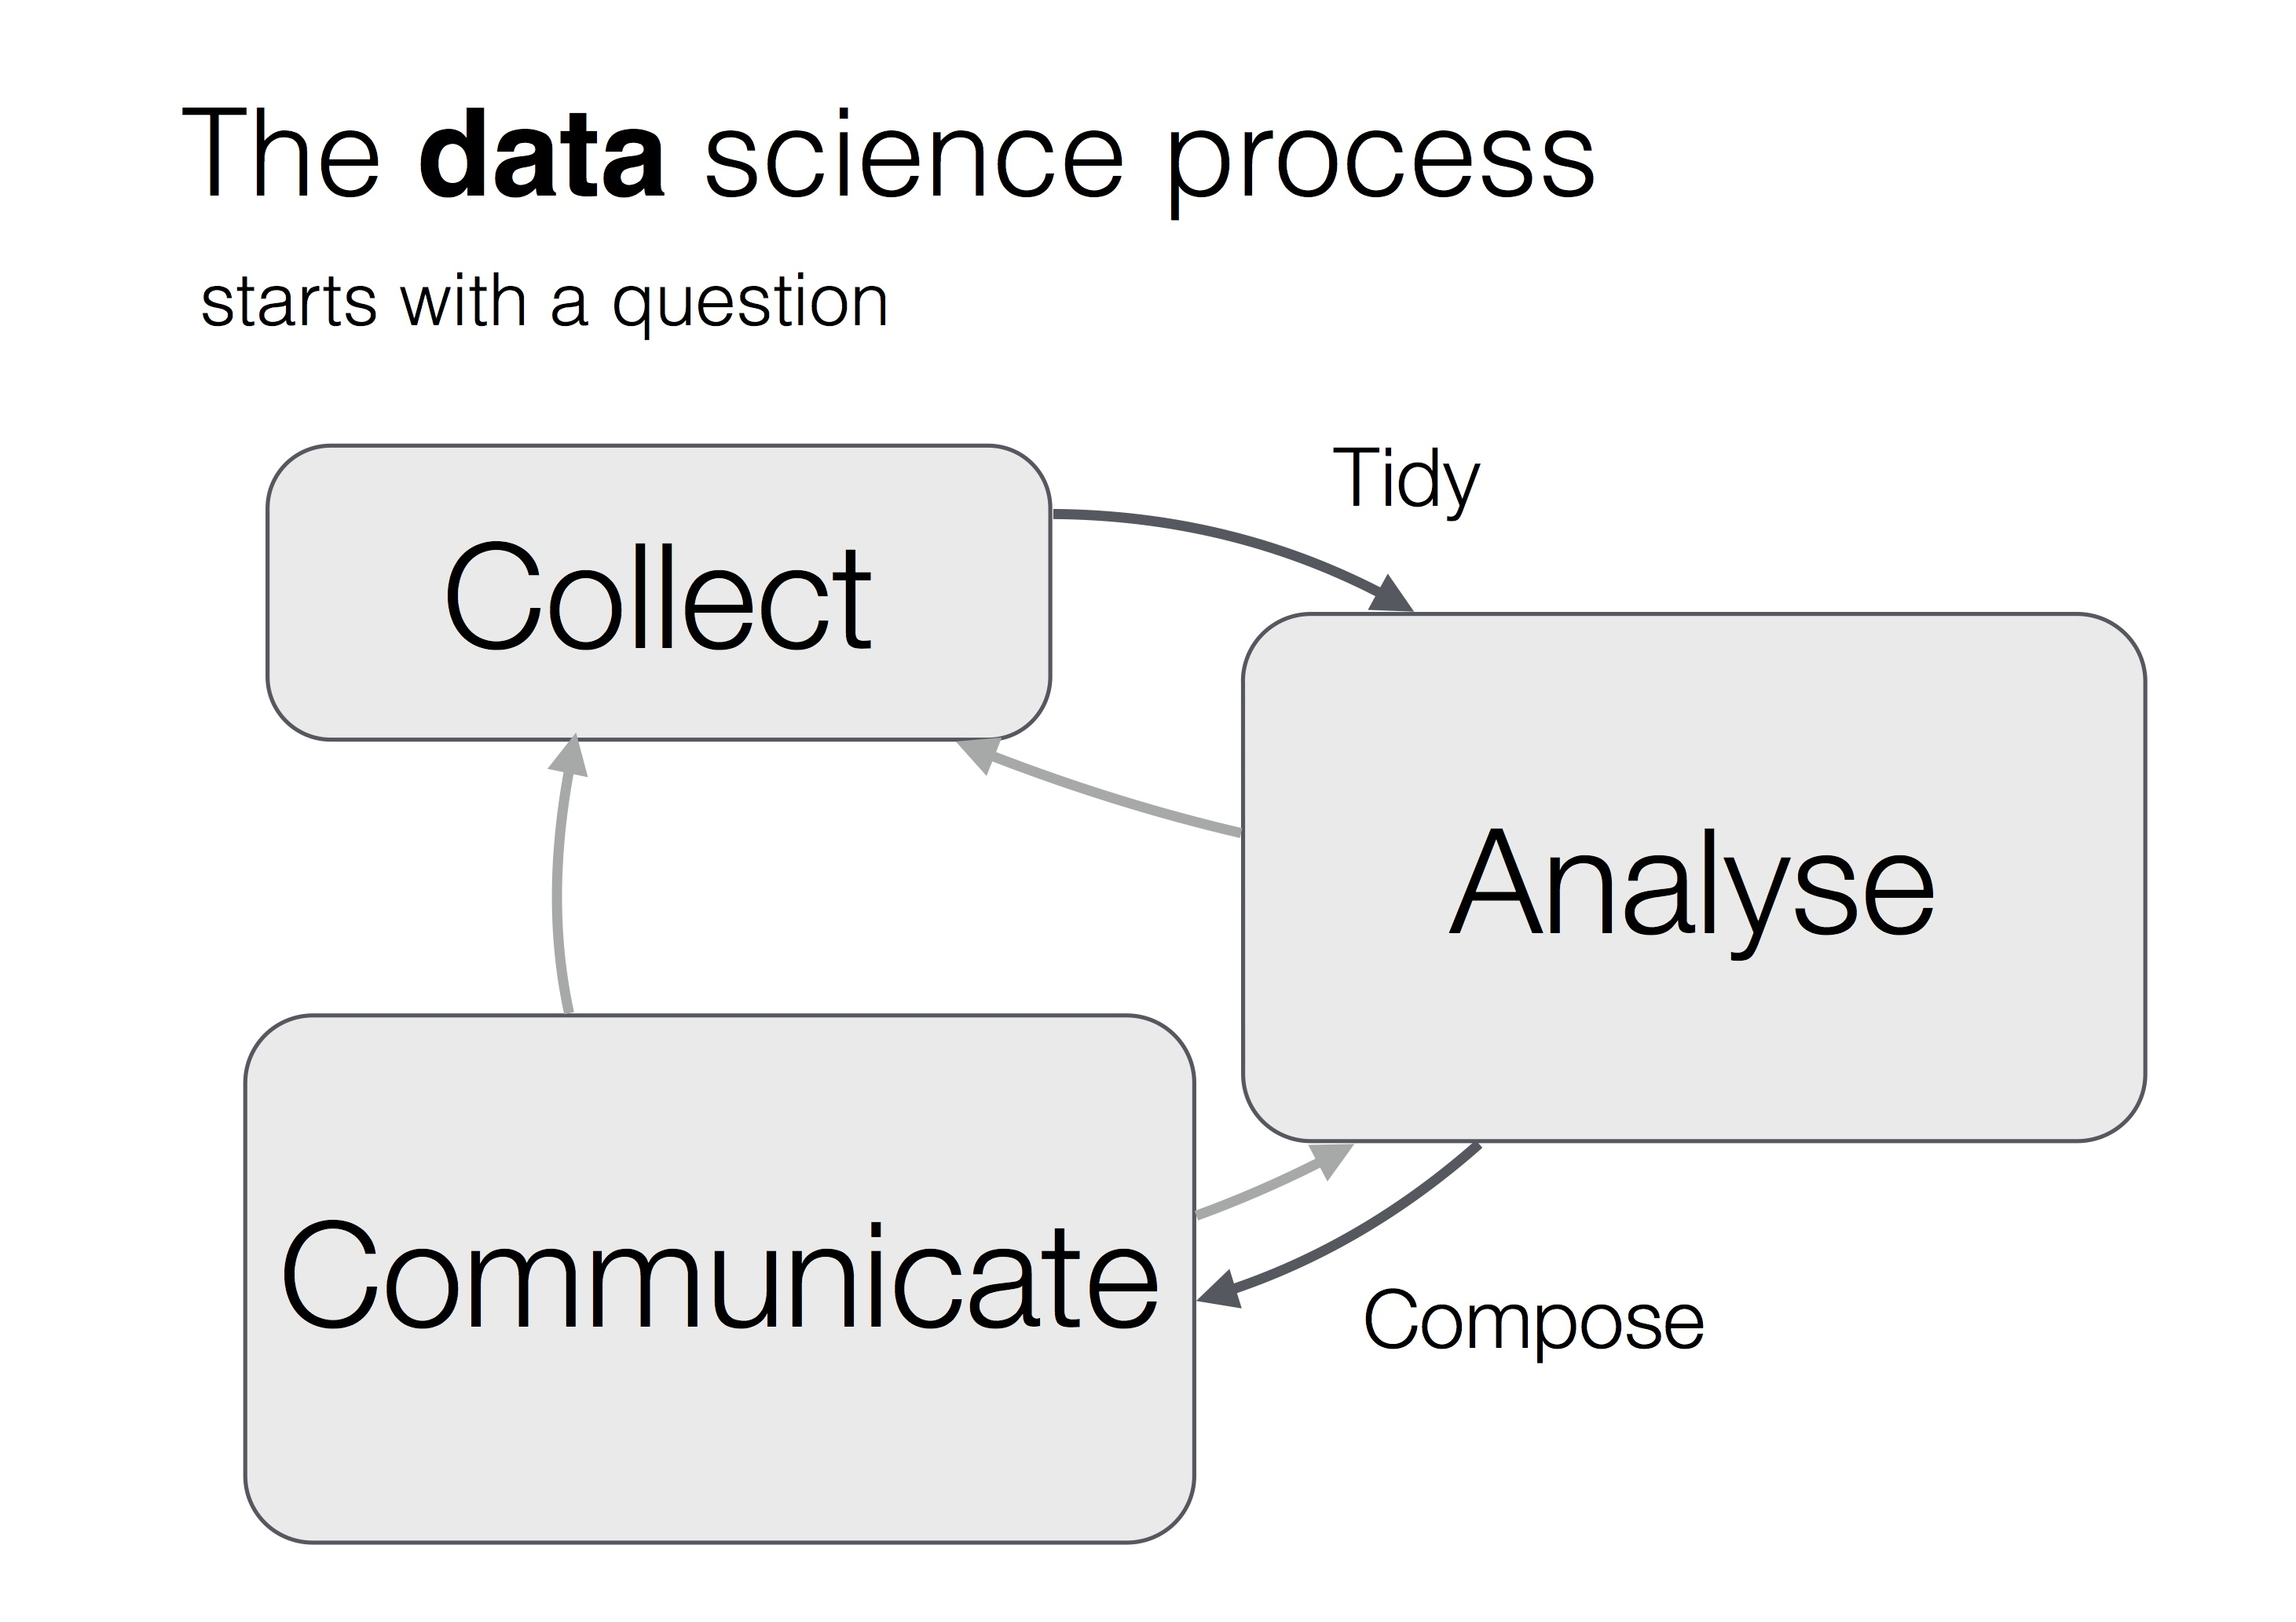
\includegraphics[height=0.8\textheight]{img/diagram02.jpg}
\end{center}

{\footnotesize diagram from Charlotte Wickham \url{http://stat511.cwick.co.nz/}}

\end{frame}

% %%%%%%%%%%%%%%%%%%%%%%%%%%%%%%%%%%%%%%%%%%%%%%%%%%%
% \begin{frame}[fragile]

% \begin{center}
% 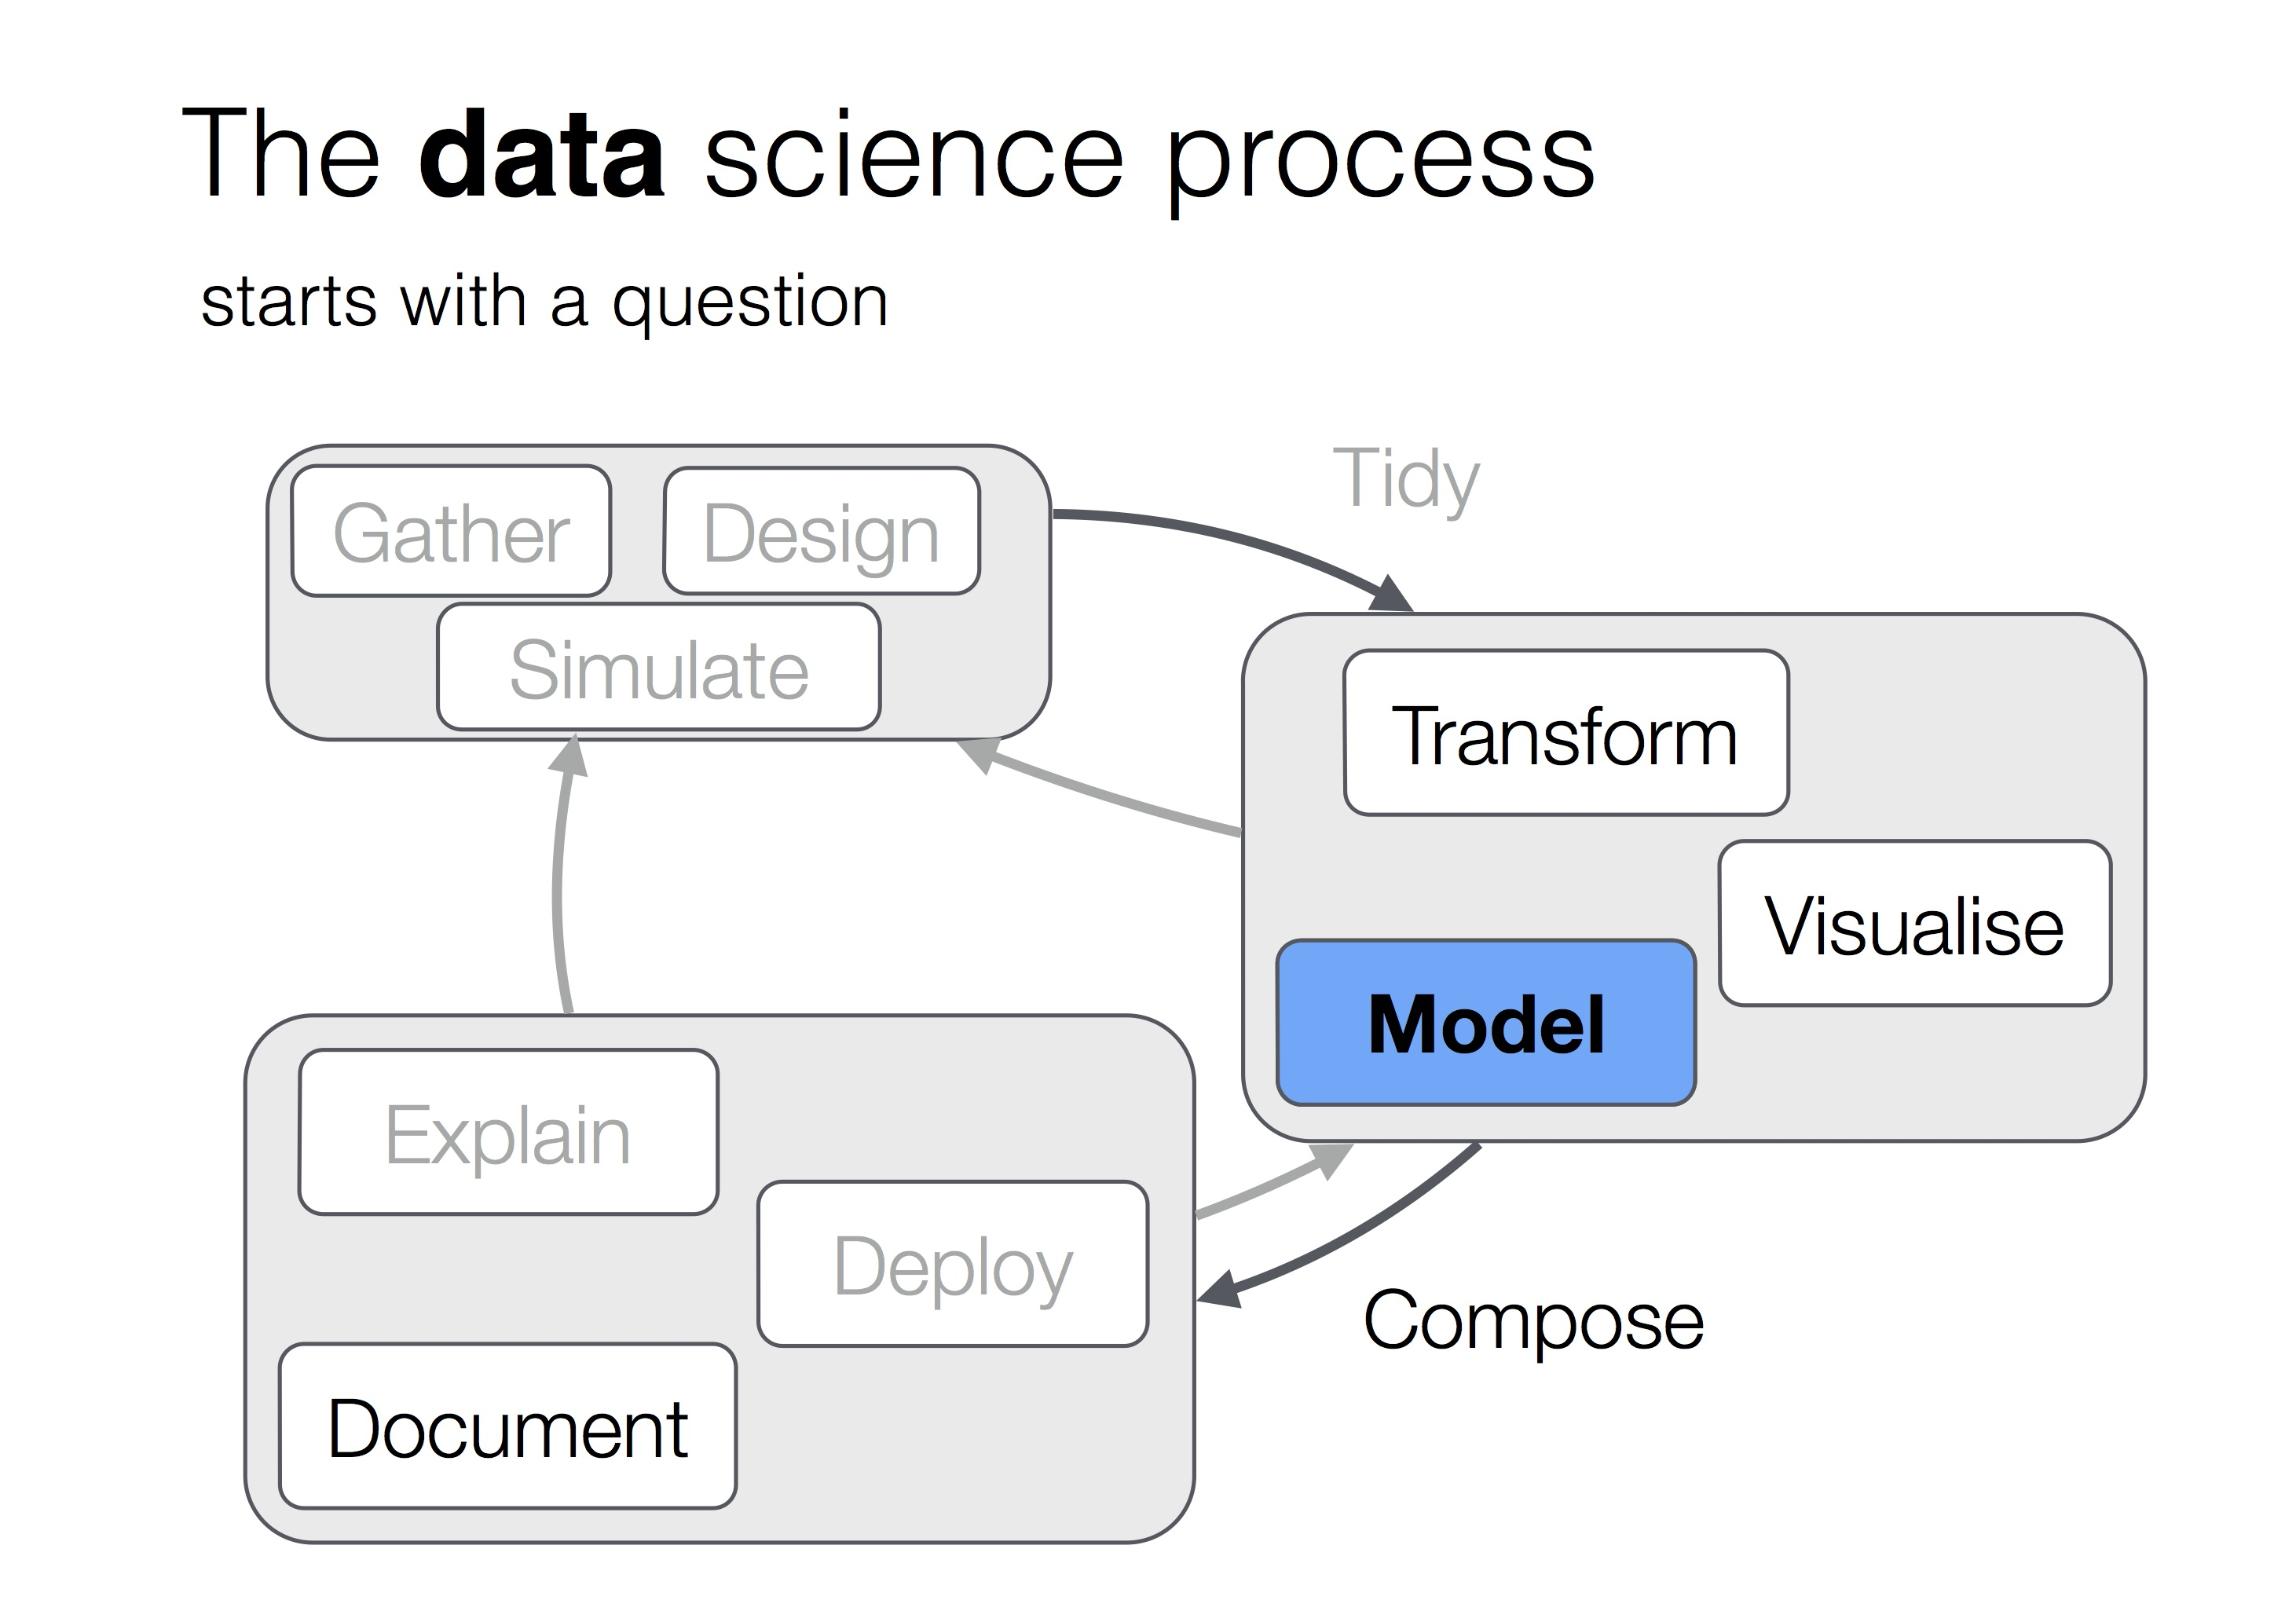
\includegraphics[height=0.8\textheight]{img/diagram03.jpg}
% \end{center}

% {\footnotesize diagram from Charlotte Wickham \url{http://stat511.cwick.co.nz/}}

% \end{frame}

% %%%%%%%%%%%%%%%%%%%%%%%%%%%%%%%%%%%%%%%%%%%%%%%%%%%
% \begin{frame}[fragile] \frametitle{}

% \stitle{Schedule:}

% First half - Applied data analysis
% \begin{itemize}
% \item {Week 01: Basics of R}
% \item {Week 02: Data visualization}
% \item {Week 03: Data manipulation}
% \item {Week 04: Model basics}
% \item {Week 05: Joining data}
% \item {Week 06: Review and midterm 1}
% \end{itemize}

% \end{frame}

% %%%%%%%%%%%%%%%%%%%%%%%%%%%%%%%%%%%%%%%%%%%%%%%%%%%
% \begin{frame}[fragile] \frametitle{}

% \stitle{Schedule (cont.):}

% Second half - Statistical inference
% \begin{itemize}
% \item {Week 07: Normality \& probability}
% \item {Week 08: Sampling distributions}
% \item {Week 09: Statistical inference (Fall break Tuesday)}
% \item {Week 10: Simple linear regression}
% \item {Week 11: Indicator variables and ANOVA}
% \item {Week 12: Linear regression}
% \item {Week 13: Review and midterm 2}
% \end{itemize}

% \end{frame}

% %%%%%%%%%%%%%%%%%%%%%%%%%%%%%%%%%%%%%%%%%%%%%%%%%%%
% \begin{frame}[fragile] \frametitle{}

% \begin{flushright}
% {\sc\fontsize{1cm}{0cm}\selectfont \textcolor{solarized@blue}{References}}
% \end{flushright}

% \end{frame}

% %%%%%%%%%%%%%%%%%%%%%%%%%%%%%%%%%%%%%%%%%%%%%%%%%%%
% \begin{frame}[fragile] \frametitle{}

% \noindent
% \begin{minipage}{0.5\textwidth}
% 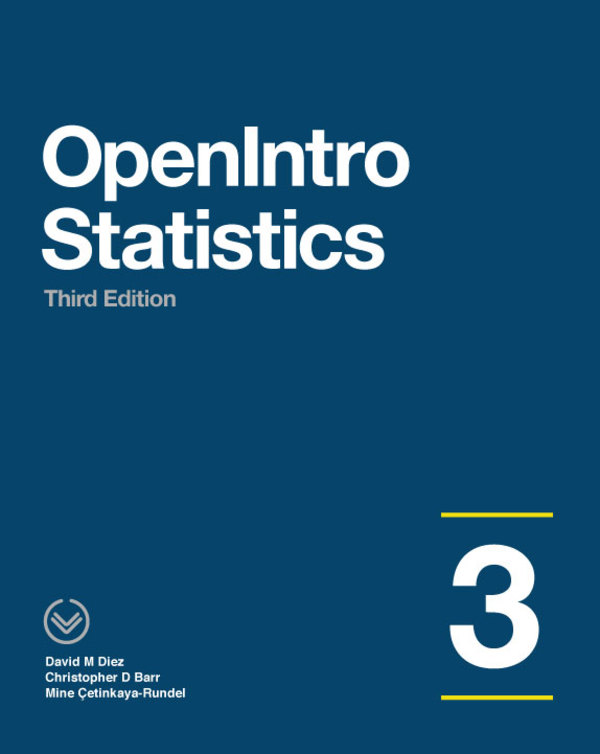
\includegraphics[width=0.9\linewidth]{img/openintro.jpg}
% \end{minipage}%%% to prevent a space
% \begin{minipage}{0.5\textwidth}\small
% David M Diez, Christopher D Barr, Mine Çetinkaya-Rundel.
% \textit{OpenIntro Statistics}. OpenIntro, Inc., Third Edition, 2015.\\

% \url{https://www.openintro.org/stat/}
% \end{minipage}

% \end{frame}

% %%%%%%%%%%%%%%%%%%%%%%%%%%%%%%%%%%%%%%%%%%%%%%%%%%%
% \begin{frame}[fragile] \frametitle{}

% \noindent
% \begin{minipage}{0.5\textwidth}
% 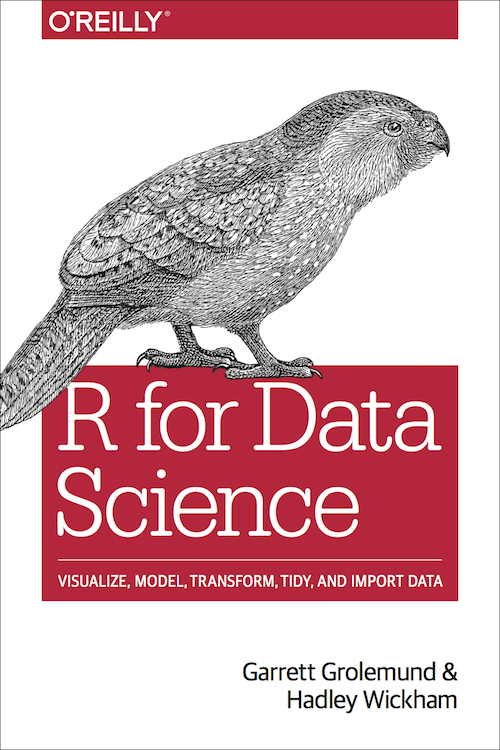
\includegraphics[width=0.9\linewidth]{img/rdatasci.png}
% \end{minipage}%%% to prevent a space
% \begin{minipage}{0.5\textwidth}\small
% Garrett Grolemund, Hadley Wickham. \textit{R for Data Science}.
% O'Reilly Media, First edition, 2016. \\

% \url{http://r4ds.had.co.nz/}.
% \end{minipage}

% \end{frame}

% %%%%%%%%%%%%%%%%%%%%%%%%%%%%%%%%%%%%%%%%%%%%%%%%%%%
% \begin{frame}[fragile] \frametitle{}

% \noindent
% \begin{minipage}{0.5\textwidth}
% 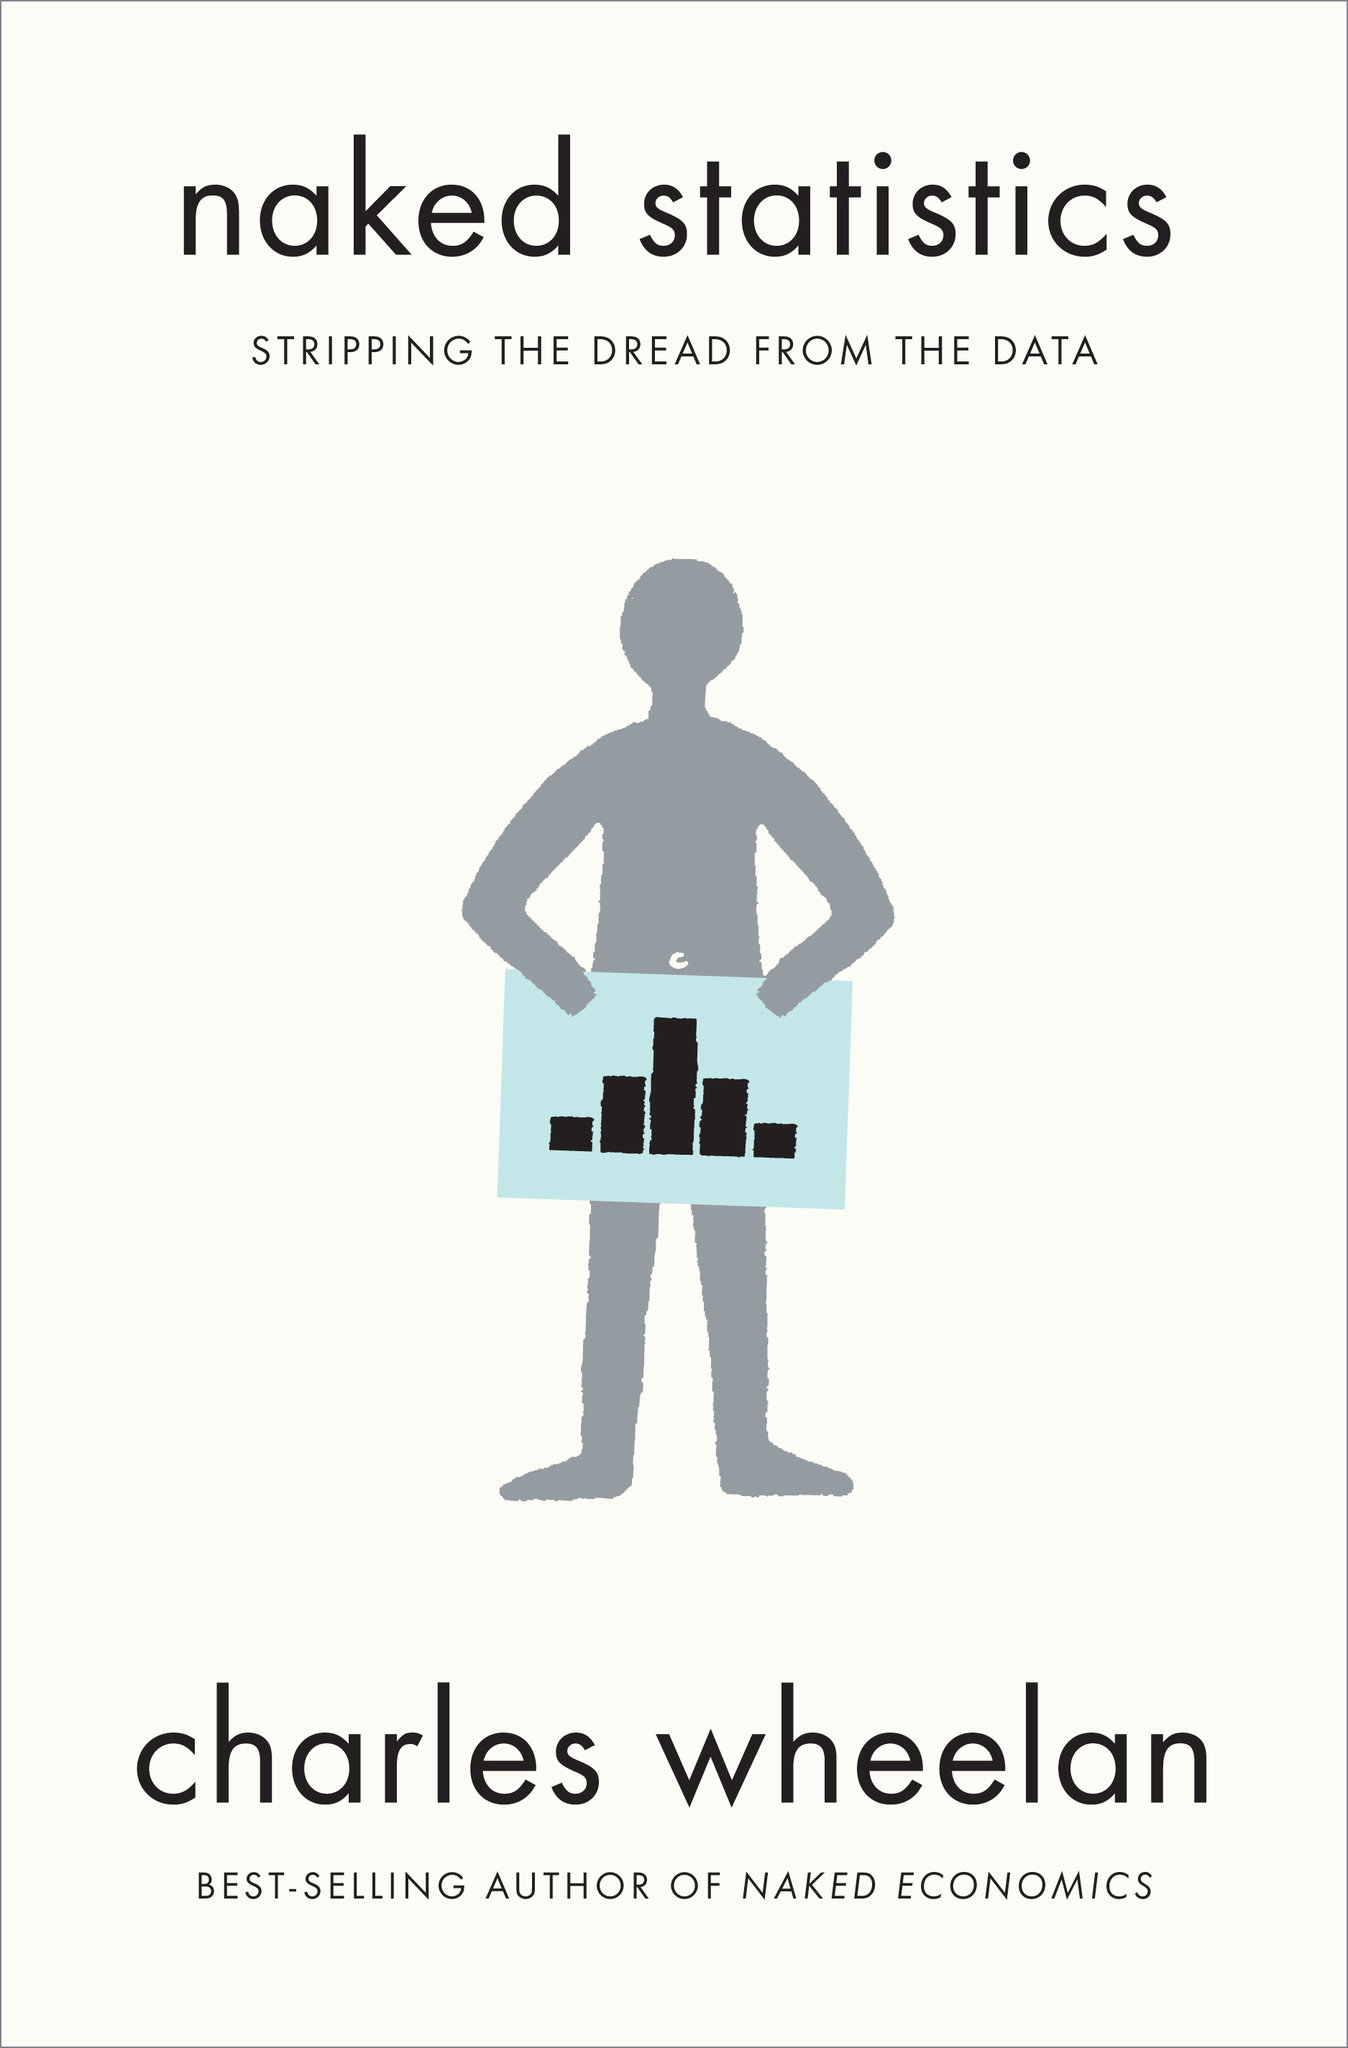
\includegraphics[width=0.8\linewidth]{img/nakedstats.jpg}
% \end{minipage}%%% to prevent a space
% \begin{minipage}{0.5\textwidth}\small
% Charles Wheelan. \textit{Naked Statistics: Stripping the Dread from the Data}. W. W. Norton \& Company, 2014.
% \end{minipage}

% \end{frame}

% %%%%%%%%%%%%%%%%%%%%%%%%%%%%%%%%%%%%%%%%%%%%%%%%%%%
% \begin{frame}[fragile] \frametitle{}

% \begin{flushright}
% {\sc\fontsize{1cm}{0cm}\selectfont \textcolor{solarized@blue}{Course policies}}
% \end{flushright}

% \end{frame}

% %%%%%%%%%%%%%%%%%%%%%%%%%%%%%%%%%%%%%%%%%%%%%%%%%%%
% \begin{frame}[fragile] \frametitle{}

% \stitle{Course materials:}

% Nearly all of the materials we use in this class will be posted on blackboard.

% \end{frame}


% %%%%%%%%%%%%%%%%%%%%%%%%%%%%%%%%%%%%%%%%%%%%%%%%%%%
% \begin{frame}[fragile] \frametitle{}

% \stitle{Final grades:}

% Every graded work in this course will be scored on a $4$ point scale,
% roughly corresponding to the $4.0$ GPA grading scheme. Your final grade
% will be calculated by taking the weighted average of all of assignments
% as follows:
% \begin{itemize}\setlength\itemsep{0em}
% \item Quizzes 20\% (best 8 of 10; 2.5\% each)
% \item Midterms 20\% (10\% each)
% \item Data analyses 30\% (10\% each)
% \item Final 30\%
% \end{itemize}
% Final grades are determined by reading off the weighted average score
% from a table matching these to letter grades.

% \end{frame}

% %%%%%%%%%%%%%%%%%%%%%%%%%%%%%%%%%%%%%%%%%%%%%%%%%%%
% \begin{frame}[fragile] \frametitle{}

% \stitle{Final grades (cont.):}

% \begin{center}
% \begin{tabular}{c || c}
% Numeric Average & \multicolumn{1}{| c}{Final Grade} \\
% \hline \hline
% 3.80 to 4.00 & A   \\
% 3.50 to 3.79 & A-  \\
% 3.20 to 3.49 & B+  \\
% 2.80 to 3.19 & B   \\
% 2.50 to 2.79 & B-  \\
% 2.20 to 2.49 & C+  \\
% 1.80 to 2.19 & C   \\
% 1.50 to 1.79 & C-  \\
% 0.00 to 1.49 & F
% \end{tabular}
% \end{center}
% Any grades on the boundaries (i.e., $3.794$) will be rounded up
% to the nearest second decimal place.

% \end{frame}

% %%%%%%%%%%%%%%%%%%%%%%%%%%%%%%%%%%%%%%%%%%%%%%%%%%%
% \begin{frame}[fragile] \frametitle{}

% \stitle{Quizzes:}

% There will be $10$ short quizzes given during the semester. These will
% be at the end of class on Tuesdays, for weeks 2-12 (one week is missing
% for Fall break). All will consist of $4$ questions, such as
% True/False, multiple choice, and matching.

% \end{frame}

% %%%%%%%%%%%%%%%%%%%%%%%%%%%%%%%%%%%%%%%%%%%%%%%%%%%
% \begin{frame}[fragile] \frametitle{}

% \stitle{Midterms and Finals:}

% We will have two midterms and one final exam. The format for all three
% will consist of completing a short data analysis using R on the computers
% in our classroom lab. You may use any external references during the exam,
% and I will provide documentation (and possibly the data itself) for the datasets
% ahead of the exam to allow you to jump right in from the start.

% \end{frame}

% %%%%%%%%%%%%%%%%%%%%%%%%%%%%%%%%%%%%%%%%%%%%%%%%%%%
% \begin{frame}[fragile] \frametitle{}

% \stitle{Midterms and Finals (cont.):}

% The dates for the exams are:
% \begin{itemize}\setlength\itemsep{0em}
% \item Midterm I: 2016-09-29
% \item Midterm II: 2016-11-17
% \item Final: 2016-12-12 (section 02) or 2016-12-13 (section 03)
% \end{itemize}
% The first will cover the basics of data manipulation and visualization. The
% second exam and final will also cover basic statistical inference and modeling.
% I plan to allow students the option of taking the final exam at an alternative
% time or in the other section's slot.

% \end{frame}

% %%%%%%%%%%%%%%%%%%%%%%%%%%%%%%%%%%%%%%%%%%%%%%%%%%%
% \begin{frame}[fragile] \frametitle{}

% \stitle{Data analyses:}

% We will also have three data analysis reports due throughout the semester. The planned
% due dates for these are as follows, though these may end up being moved slightly:
% \begin{itemize}\setlength\itemsep{0em}
% \item 2016-09-15
% \item 2016-11-03
% \item 2016-12-02
% \end{itemize}
% The format will be similar to the exams, where you are given a dataset and some
% leading questions to answer, but will be completed out of class.
% As these are not completed under any time pressure, the level of polish should exceed
% that of the exams.

% \end{frame}


% %%%%%%%%%%%%%%%%%%%%%%%%%%%%%%%%%%%%%%%%%%%%%%%%%%%
% \begin{frame}[fragile] \frametitle{}

% \stitle{Late Policy:}

% Students are expected to submit work in on-time and to take quizzes when they
% are scheduled. If there are any issues with this, please let me know as soon
% as possible. I will only accept late assignments in the event of exceptional
% circumstances (such as extended absences or family emergencies). There are no
% make-up exams.

% \end{frame}

% %%%%%%%%%%%%%%%%%%%%%%%%%%%%%%%%%%%%%%%%%%%%%%%%%%%
% \begin{frame}[fragile] \frametitle{}

% \stitle{Class Participation:}

% This course will be very interactive. Your attendance in class and
% full engagement with the material are both expected, though you will
% not be penalized for missing class unless (following a warning) they
% become excessive. This may result in a grade of V.

% \end{frame}

% %%%%%%%%%%%%%%%%%%%%%%%%%%%%%%%%%%%%%%%%%%%%%%%%%%%
% \begin{frame}[fragile] \frametitle{}

% \stitle{Special approval requests:}

% If you have special approval forms for extra time on exams or any other
% special circumstances, please speak with me as early as possible.

% \end{frame}

% %%%%%%%%%%%%%%%%%%%%%%%%%%%%%%%%%%%%%%%%%%%%%%%%%%%
% \begin{frame}[fragile] \frametitle{}

% \stitle{Academic Integrity:}

% Cheating and plagiarism are grave scholarly offenses and potential grounds
% for expulsion; they are also a major barrier to your intellectual development.
% You are expected to familiarize yourself with the entirety of the
% University of Richmond’s Honor Code. If you are confused or unsure about
% appropriate citation protocol or any other aspect of the Honor code,
% please consult me before turning in an assignment.

% \end{frame}

% %%%%%%%%%%%%%%%%%%%%%%%%%%%%%%%%%%%%%%%%%%%%%%%%%%%
% \begin{frame}[fragile] \frametitle{}

% \stitle{Data collection:}

% From time to time, I will be collecting data from the class either through
% online polls or live in class. I try my best to ask questions that are neither
% overly personal or sensitive. If at any point you ever feel uncomfortable
% answering something, however, feel free to `pass' or simply make up an answer.

% \end{frame}


%%%%%%%%%%%%%%%%%%%%%%%%%%%%%%%%%%%%%%%%%%%%%%%%%%%
\begin{frame}[fragile] \frametitle{}

\begin{flushright}
{\sc\fontsize{1cm}{0cm}\selectfont \textcolor{solarized@blue}{Course Outline}}
\end{flushright}

\end{frame}

%%%%%%%%%%%%%%%%%%%%%%%%%%%%%%%%%%%%%%%%%%%%%%%%%%%
\begin{frame}[fragile] \frametitle{}

\stitle{First Half}

\begin{itemize}
\item `labs': daily work to be handed in on box before the next
  class period; graded on pass/fail scale
\item `midterms': two open notes, in-class midterms resembling the
  labs
\end{itemize}

\end{frame}

%%%%%%%%%%%%%%%%%%%%%%%%%%%%%%%%%%%%%%%%%%%%%%%%%%%
\begin{frame}[fragile] \frametitle{}

\stitle{Second Half}

You will complete $4$ additional data analyses.
These analyses will come from one of six \textit{thematic
tracts}:

\begin{itemize}\setlength\itemsep{0em}
\item public policy
\item spatial analysis
\item healthcare and sciences
\item sports
\item business
\item culture
\end{itemize}

\end{frame}

%%%%%%%%%%%%%%%%%%%%%%%%%%%%%%%%%%%%%%%%%%%%%%%%%%%
\begin{frame}[fragile] \frametitle{}

{\fontsize{0.6cm}{0cm}\selectfont \blue{Questions?} }

\end{frame}

\end{document}













